\documentclass[12pt]{beamer}

%Paquetes instalados%

\usepackage[utf8]{inputenc} %Paquetes para idioma y caracteres españoles
\usepackage[spanish]{babel} %Paquetes para idioma y caracteres españoles
\usepackage{ragged2e} %Justificar texto%

%Comandos e instrucciones%
\usetheme{Madrid}
\title{Medieval Game}
\subtitle{Diagramas de clase}
\author{Juan, Alejandro, Pedro, Raul, Antonio}
\date{\today}
\logo{
\includegraphics[scale=0.15]{logo.png}}
\institute[]{
    \inst{}IES Francisco de los Ríos \newline
    \inst{}1º CSFP Desarrollo de Aplicaciones Multiplataforma \newline
    \inst{}Sistemas Informáticos

}

\AtBeginSection[]
{
    \begin{frame}
        \frametitle{Tabla de Contenidos}
        \tableofcontents[currentsection]
    \end{frame}
}

\AtBeginSubsection[]
{
    \begin{frame}
        \frametitle{Tabla de Contenidos}
        \tableofcontents[currentsection,currentsubsection]
    \end{frame}
}


\begin{document}

    \begin{frame}
        \maketitle
    \end{frame}

    \begin{frame}
        \begin{figure}[H]
            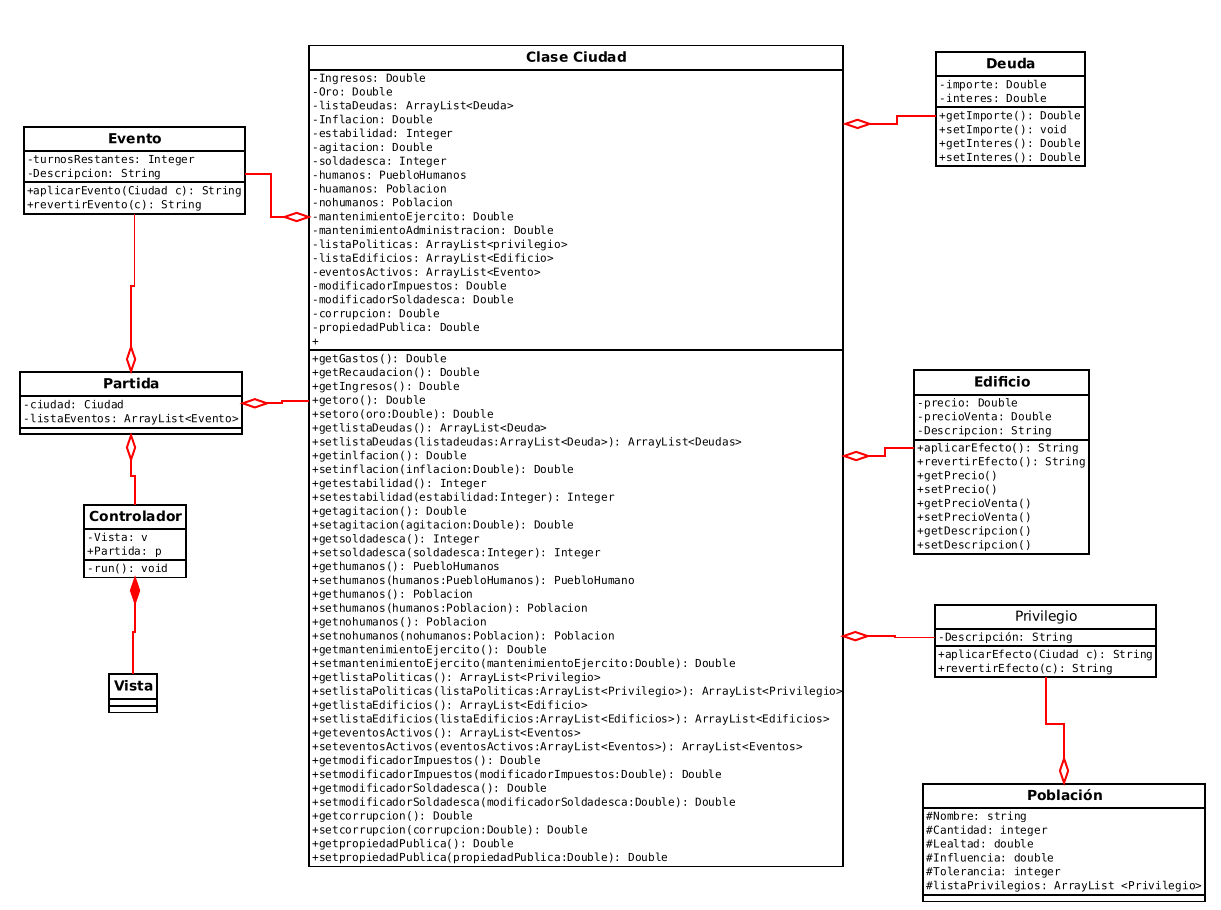
\includegraphics[width=\textwidth]{Diagrama.png}
        \end{figure}
    \end{frame}
    \begin{frame}
        \frametitle{Requisitos pedidos}
        \framesubtitle{Turnos}
       \begin{itemize}
            \item El juego consiste en aguantar todos los turnos que se pueda sin que ningún desastre pase en la ciudad.
            \item A medida que pasan los turnos diferentes parámetros de la ciudad van empeorando, por ejemplo la inflación.
            \item El jugador puede tomar medidas sobre éstos inconvenientes pero la mayoría de eventos serán negativos.
        \end{itemize} 
    
    \end{frame}

    \begin{frame}
        \frametitle{Requisitos pedidos}
        \framesubtitle{Turnos}
       \begin{itemize}
            \item Al final de cada turno se lanzará un evento aleatorio, la mayoría de caracter eminentemente negativo. 
            \item Además si se cumplen ciertas condiciones como muchas deudas, nivel de agitación alto o mucha corrupción se activará un desastre. 
            \item Si no se palia éste desastre durante unos turnos determinados se terminará la partida.
        \end{itemize} 
        
    \end{frame}

    \begin{frame}
        \frametitle{Requisitos pedidos}
        \framesubtitle{Turnos}
        \begin{itemize}
            \item Durante el turno podremos tomar decisiones tales como dar y quitar privilegios, endeudarnos, pagar deudas, cambiar el mantenimiento del ejercito, etc
            \item Así mismo podremos consultar el estado de la ciudad antes de que finalize el turno.
        \end{itemize}
        
    \end{frame}

    \begin{frame}
        \frametitle{Requisitos pedidos}
        \framesubtitle{Edificios}
        \begin{itemize}
            \item En lugar de la creación de 2 edificios cada domingo, se implementará un sistema de edificios los cuales han de pagarse con dinero.
            \item Éstos edificios tendrán efectos positivos, como reducción de la inflación cada turno, más generación de dinero, menos agitación.
        \end{itemize}
        
    \end{frame}
    
    \begin{frame}
        \frametitle{Requisitos pedidos}
        \framesubtitle{Sistema de clases}
        \begin{itemize}
            \item Tenemos dos estamentos los cuales tenemos que controlar como gobernantes: humanos y no humanos;
            \item Cada población tiene cierta influencia y lealtad. Si éstos valores se salen de control se produce un desastre. 
            \item La población va creciendo lentamente y producen oro y soldados para el gobernante. 
        \end{itemize}
        
    \end{frame}

    \begin{frame}
        \frametitle{Requisitos pedidos}
        \framesubtitle{Sistema de clases}
        \begin{itemize}
            \item Podemos asignar privilegios a éstos estamentos, los cuales dan beneficios, pero a costa de influencia o lealtad. 
            \item Para poder eliminar un privilegio la lealtad debe ser mayor a la influencia, y ésto causará perdida de lealtad. 
            \item Cada población tendrá un porcentaje del total de propiedades de la ciudad. 
            \item Dependiendo de éste porcentaje la población tendrá unos determinados efectos.
        \end{itemize}
        
    \end{frame}

    \begin{frame}
        \frametitle{Requisitos pedidos}
        \framesubtitle{Sistema de clases}
        \begin{itemize}
            \item El propio gobernante puede tener privilegios y también tiene posesiones. 
            \item Si el gobernante tiene poca propiedad sufrirá severas penalizaciones. 
            \item Los privilegios del gobernante serán dificiles de adquirir pero muy poderosos.
        \end{itemize}
        
    \end{frame}
\end{document}